\documentclass[tikz]{standalone}
\usetikzlibrary{positioning}
% newcommands.tex

\newcommand{\enq}{\texttt{enq}}
\newcommand{\deq}{\texttt{deq}}
\newcommand{\pput}{\texttt{PUT}}
\newcommand{\get}{\texttt{GET}}
\newcommand{\vs}{\texttt{vis}}
\newcommand{\so}{\texttt{so}}
\newcommand{\arb}{\texttt{ar}}
\newcommand{\rf}{\texttt{rf}}

% example
\newcommand{\po}[2]{\draw [->, thick] (#1) to node[above] {\Large{\so}} (#2);}
\newcommand{\pva}[2]{\draw [->, thick] (#1) to node[above] {$\Large{\so},\Large{\vs},\Large{\arb}$} (#2);}
\newcommand{\pbva}[2]{\draw [->, thick] (#1) to node[above] {$\Large{\so}$} node[below] {$\Large{\vs},\Large{\arb}$} (#2);}
\newcommand{\pv}[2]{\draw [->, thick] (#1) to node[above] {\Large{\so}} node[below] {\Large{\vs}} (#2);}
\newcommand{\evis}[2]{\draw [->, thick] (#1) to node[above, sloped, near end] {\Large{\vs}} (#2);}
\newcommand{\mvis}[2]{\draw [->, thick] (#1) to node[above, sloped] {\Large{\vs}} (#2);}
\newcommand{\ar}[2]{\draw [->, thick, allow upside down] (#1) to node[above, sloped] {\Large{\arb}} (#2);}
\newcommand{\va}[2]{\draw [->, thick, allow upside down] (#1) to node[above, sloped] {$\Large{\vs},\Large{\arb}$} (#2);}
\newcommand{\vab}[2]{\draw [->, thick, allow upside down] (#1) to node[below, sloped, near end] {$\Large{\vs},\Large{\arb}$} (#2);}
\newcommand{\vae}[2]{\draw [->, thick, allow upside down] (#1) to node[above, sloped, near end] {$\Large{\vs},\Large{\arb}$} (#2);}
\newcommand{\vas}[2]{\draw [->, thick, allow upside down] (#1) to node[sloped, near start, above] {$\Large{\vs},\Large{\arb}$} (#2);}

% serialization
\newcommand{\scc}[2]{\draw [->, very thick] (#1) to (#2);}
\newcommand{\rva}[2]{\draw [->, thick, allow upside down] (#1) to node[above, sloped] {$\Large{\rf},\Large{\vs},\Large{\arb}$} (#2);}
\newcommand{\rvb}[2]{\draw [->, thick, allow upside down] (#1) to node[below, sloped] {$\Large{\rf},\Large{\vs},\Large{\arb}$} (#2);}


\renewcommand{\vae}[2]{\draw [->, thick, allow upside down] (#1) to node[below, sloped, pos=0.83] {$\Large{\vs},\Large{\arb}$} (#2);}
\renewcommand{\vab}[2]{\draw [->, thick, allow upside down] (#1) to node[below, sloped, pos=0.4] {$\Large{\vs},\Large{\arb}$} (#2);}
\renewcommand{\va}[2]{\draw [->, thick, allow upside down] (#1) to node[above, sloped, pos=0.7] {$\Large{\vs},\Large{\arb}$} (#2);}
\newcommand{\vaa}[2]{\draw [->, thick, allow upside down] (#1) to node[above, sloped, pos=0.6] {$\Large{\vs},\Large{\arb}$} (#2);}

\begin{document}
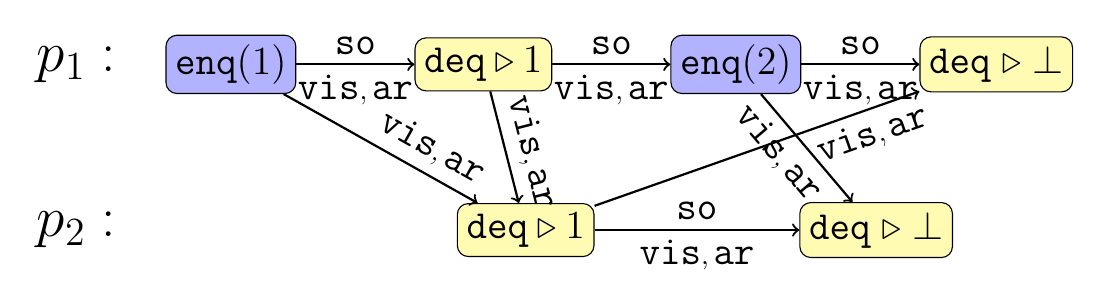
\begin{tikzpicture}
\tikzset{
  enq-op/.style = {rectangle, rounded corners, fill = blue!30, draw, font = \Large},
  deq-op/.style = {rectangle, rounded corners, fill = yellow!30, draw, font = \Large},
  process/.style = {font = \huge},
  po/.style = {->, very thick},
  vis/.style = {->, shorten >= 3pt, very thick, dashed}
}

  \node (p1) [process] {$p_1:$};
  \node (p1-enq1) [enq-op, right = 0.5cm of p1] {$\enq(1)$};
  \node (p1-deq1) [deq-op, right = 1.5cm of p1-enq1] {$\deq\triangleright1$};
  \node (p1-enq2) [enq-op, right = 1.5cm of p1-deq1] {$\enq(2)$};
  \node (p1-deq0) [deq-op, right = 1.5cm of p1-enq2] {$\deq\;\triangleright\perp$};

  \node (p2) [process, below = 1.4cm of p1] {$p_2:$};
  \node (p2-deq1) [deq-op, right = 4.2cm of p2] {$\deq\triangleright1$};
  \node (p2-deq0) [deq-op, right = 2.6cm of p2-deq1] {$\deq\;\triangleright\perp$};

  \pbva{p1-enq1}{p1-deq1};
  \pbva{p1-deq1}{p1-enq2};
  \pbva{p1-enq2}{p1-deq0};
  \pbva{p2-deq1}{p2-deq0};

  \va{p1-enq1}{p2-deq1};
  \vaa{p1-deq1}{p2-deq1};
  \vab{p1-enq2}{p2-deq0};
  \vae{p2-deq1}{p1-deq0};

\end{tikzpicture}
\end{document}
